\subsection{Hasil dan Perbandingan dengan \textit{Scikit-learn}}
\label{subsec:knn-hasil}

Model terpilih dibandingkan dengan \texttt{sklearn.neighbors.KNeighborsClassifier} \cite{pedregosa2011sklearn} pada \textbf{data holdout yang sama}. Kedua implementasi menerima matriks 26 kolom yang sama dari \textit{preprocessor} yang hanya di-\textit{fit} pada development. Parameter pembanding disamakan, yaitu $k=7$, Manhattan, bobot \textit{uniform}, dan pencarian \textit{brute force}. Dengan demikian, pengujian memeriksa konsistensi hasil prediksi implementasi \textit{from scratch}, bukan perbedaan akibat pemrosesan data.

\begin{table}[H]
 \centering
 \caption{Perbandingan performa KNN pada 5.462 reservasi \textit{holdout}}
 \label{tab:knn-hasil}
 \begin{tabular}{l c c c c}
  \toprule
  \textbf{Implementasi} & \textbf{Macro F1} & \textbf{Accuracy} & \textbf{Macro Precision} & \textbf{Macro Recall} \\
  \midrule
  \textit{From scratch} & 0,82830 & 0,85244 & 0,83803 & 0,82075 \\
  \textit{Scikit-learn} & 0,82830 & 0,85244 & 0,83803 & 0,82075 \\
  \bottomrule
 \end{tabular}
\end{table}

\textbf{Seluruh 5.462 prediksi identik} antara kedua implementasi, sehingga kesesuaian label mencapai 100\%. Confusion matrix keduanya sama, sebagaimana ditampilkan pada Gambar~\ref{fig:knn-cm}. Hasil ini mendukung ketepatan implementasi jarak dan suara mayoritas pada konfigurasi serta data yang diuji. Kesamaan prediksi tersebut tidak berarti seluruh kemungkinan \textit{tie} jarak akan selalu ditangani identik oleh kedua implementasi.

\begin{figure}[H]
 \centering
 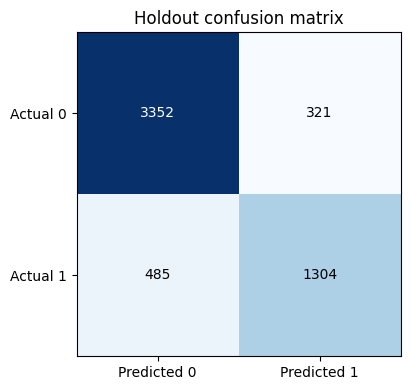
\includegraphics[width=0.66\textwidth]{knn/knn_confusion_matrix.png}
 \caption{\textit{Confusion matrix} KNN \textit{from scratch} pada \textit{holdout}, identik dengan \textit{scikit-learn}}
 \label{fig:knn-cm}
\end{figure}

\subsubsection{Analisis}
Dari 3.673 reservasi yang sebenarnya tidak dibatalkan, model mengklasifikasikan 3.352 dengan benar dan menghasilkan 321 \textit{false positive}. Dari 1.789 reservasi yang dibatalkan, model mengenali 1.304 dengan benar dan melewatkan 485 sebagai \textit{false negative}. \textit{Recall} kelas batal sebesar 0,72890 lebih rendah daripada kelas tidak batal sebesar 0,91261. Dengan demikian, kelemahan utama KNN pada \textit{holdout} adalah pembatalan yang tidak terdeteksi, bukan ketidakcocokan implementasi dengan pustaka.

Skor Macro F1 \textit{holdout} sebesar 0,82830 sedikit di atas rata-rata CV development 0,82126. Keduanya berada pada kisaran yang sebanding, meskipun berasal dari skema evaluasi berbeda. Peningkatan kemampuan mengenali kelas batal berpotensi dilakukan melalui kalibrasi ambang keputusan atau pembobotan fitur, tetapi perubahan tersebut tidak diterapkan pada model utama. Dalam konteks bonus biaya kesalahan, FP justru memiliki konsekuensi lebih mahal sehingga arah penyesuaian keputusan juga berbeda, seperti dibahas pada Subbab~\ref{subsec:knn-bonus}.

Pengukuran waktu prediksi tidak dilakukan sebagai eksperimen pembanding, sehingga tidak ditarik kesimpulan mengenai kecepatan kedua implementasi. Versi \textit{from scratch} memakai \texttt{cdist} dan \texttt{argpartition} dengan \textit{batch} untuk membatasi memori sementara. Pembanding \textit{scikit-learn} secara eksplisit memakai \textit{brute force} agar metode pencarian tetangganya sebanding.